\documentclass[a4j,12pt]{jarticle}
\setlength{\textwidth}{170mm}
\setlength{\textheight}{260mm}
\setlength{\oddsidemargin}{-5mm}
\setlength{\topmargin}{-25mm}
\usepackage[dvipdfmx]{graphicx}
\usepackage{here}
\usepackage{theorem}
\usepackage{amsmath}
\usepackage{amsfonts}
\usepackage{ascmac}
\usepackage{bm}
\usepackage{comment}
\usepackage{listings,jlisting}

\newtheorem{theo}{定理}[section]
\newtheorem{defi}{定義}[section]
\newtheorem{lemm}{命題}[section]

\title{ベイジアンネットワークによるアンサンブル学習}   %タイトル
\author{小坪琢人}   %著者
\date{\today}   %日付

\makeatletter
\def\theequation{\thesection.\arabic{equation}}   %数式番号を(章.式)形式
\@addtoreset{equation}{section}
\def\thefigure{\thesection.\arabic{figure}}   %図番号を(章.図)形式
\@addtoreset{figure}{section}
\def\thetable{\thesection.\arabic{table}}   %表番号を(章.表)形式
\@addtoreset{table}{section}
\def\tr{\mathop{\operator@font tr}\nolimits}
\def\grad{\mathop{\operator@font grad}\nolimits}
\def\St{\mathop{\operator@font St}\nolimits}
\def\Hess{\mathop{\operator@font Hess}\nolimits}
\def\D{\mathop{\operator@font D}\nolimits}
\def\sym{\mathop{\operator@font sym}\nolimits}
\makeatother

\setlength\textheight{230mm}   %テキスト高さ
\setlength\textwidth{160mm}   %テキスト幅
\setlength{\oddsidemargin}{0mm}   %余白

\begin{document}
\maketitle   %タイトルを付ける
\setlength{\baselineskip}{20pt}   %行間幅
\pagenumbering{roman}   %目次ページ番号のスタイル
\tableofcontents   %目次を付ける
\listoffigures   %図目次を付ける
\listoftables   %表目次を付ける
\clearpage   %目次と本文を分ける
\pagenumbering{arabic}   %本文ページ番号のスタイル

%%%%%これ以下, 本文%%%%%

\section{はじめに}

現在、様々な分類手法が存在するが、

\section{理論}

\section{解析データ}

\section{結果}

\section{まとめと今後の課題}

\section{謝辞}

ベイジアンネットワークの主な性質は以下の4つが挙げられる。

グラフィカルモデル/有向かつ非巡回なグラフ/ナイーブベイズモデルの発展形/決定木モデルの特殊系

ベイズの定理とベイズ推論に基づく、グラフィカルモデルである。ベイズの定理は式$(\ref{eq:eq1})$で表され、$H$はHypothesis、$E$はEvidence、$c$はbackground contextを意味する。ベイズの定理の重要な利用として chain ruleがあり式$(\ref{eq:eq2})$で表される。

\begin{equation}
\label{eq:eq1}
P(H|E,c) = \frac{P(H|c) \times P(E|H,c)}{P(E|c)}
\end{equation}

\begin{equation}
\label{eq:eq2}
P(X_1, \ldots, X_n|c) = \prod_{i=1}^n P(X_i|X_1, \ldots, X_{i-1},c)
\end{equation}

これらの定義式はベイジアンネットワークのパラメータ学習の際に用いられる。そのため確率変数は離散値でなければならないが、境界値分類などで連続変数を離散化することで適用可能である。

\section{ベイジアンネットワークによる分類}

分類はクラスラベルを割り当てる作業に相当する。訓練データによって各クラスにおけるそれぞれの変数の条件付確率を計算し、テストデータにあてはめる。ベイズの定理によって求めた確率が最も大きくするものがクラスラベルの予測となる。最も簡単な分類器がナイーブベイズ分類であり、これは各変数間の独立性を仮定したものである。その例を図$\ref{fig:fig1}$に示す。また変数間に関係性を含めたものを Tree Augmented Naive Bayes(TAN) と呼ぶ。その例を図$\ref{fig:fig2}$に示す

\begin{figure}[H]
\begin{minipage}{0.5\hsize}
 \begin{center}
  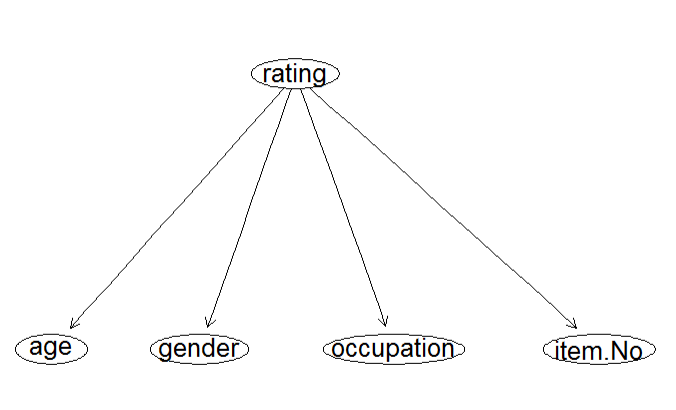
\includegraphics[width=80mm]{data/sample1.png}
 \end{center}
 \caption{ナイーブベイズの例}
 \label{fig:fig1}
 \end{minipage}
\begin{minipage}{0.5\hsize}
 \begin{center}
  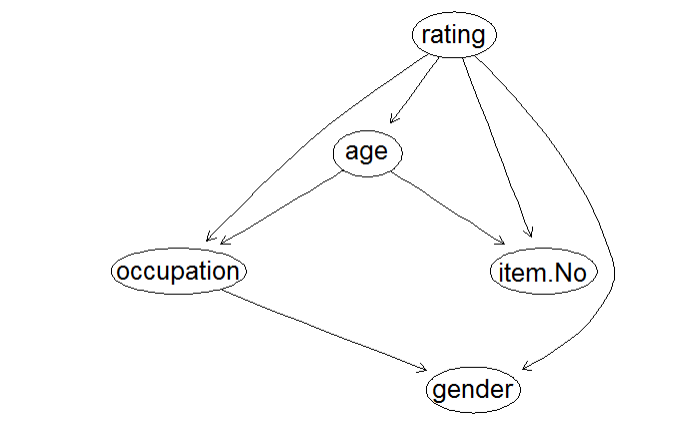
\includegraphics[width=80mm]{data/sample2.png}
 \end{center}
 \caption{ベイジアンネットワークの例}
 \label{fig:fig2}
 \end{minipage}
\end{figure}

ベイジアンネットワークには構造学習とパラメータ学習の2つのフェーズがある。それらについて説明していく。

\subsection{構造学習}

上記の通りナイーブベイズは構造がすでに決まっているので、構造学習は行わない。TANではまずナイーブベイズの構造から始まり、関係性の強い説明変数間に有向辺を加えていく。

その際、説明変数間に以下の仮定を満たす必要がある。

\begin{itemize}
\item 閉路が存在しない

\item 全ての点の入次数は1以下である

\item $n$個の説明変数に対して、$n-1$本の有向辺が存在する
\end{itemize}

関係性の強い説明変数については相互情報量をもとに決定していく。その際、元のクラスラベルの値を条件とした条件付相互情報量を用いる。ここでは条件付相互情報量を上記の仮定の下で最大化する。

\begin{eqnarray*}
\mbox{相互情報量} &=& I(X, Y) \\
\mbox{条件付相互情報量} &=& I(X, Y | C)
\end{eqnarray*}

ここで条件付相互情報量をエントロピーの式で表すと以下のように表せる。

\begin{eqnarray*}
I(X, Y | C) &=& H(X|C) - H(X|Y, C) \\
               &=& H(X, C) + H(Y, C) - H(X, Y, C) - H(C)
\end{eqnarray*}

エントロピーは以下の式で求められる。$p(x)$は各変数の取りうる値の出現確率を表している。

\begin{eqnarray*}
H(X) &=& - \sum_x p(x) \log p(x) \\
H(X, C) &=& - \sum_x \sum_c p(x) p(c) \log p(x) \log p(c)
\end{eqnarray*}

上記の例に対して条件付相互情報量を求める。結果を以下に示す。

\begin{table}[H]
\begin{center}
\caption{条件付相互情報量}
\begin{tabular}{|c||c|c|c|c|} \hline  
& age & gender & occupation & item.No \\ \hline \hline
age & 3.666 & 0.0618 & \bf{0.873} & \bf{0.981} \\
gender &  & 0.573 & \bf{0.0988} & 0.0644 \\
occupation &  &  & 2.583 & 0.517 \\
item.No &  &  &  & 6.564 \\ \hline
\end{tabular}
\end{center}
\end{table}

実際に有向辺を与える部分を太字で強調した。表からわかるように (ocupation, item.No)間のほうが値が大きいがここに線を引くと閉路ができてしまうのでその次に大きい値を用いていることがわかる。

これらの手順により相互情報量をもとに無向辺を与える。ここで相互情報量をもとに有向辺を与えることができないことに注意する。有向辺を決定するのは上記の条件のうち2つ目を用いてベイジアンネットワークを構成する。

$\Rightarrow$ 因果関係から判断しているのかは微妙であると思った。

\subsection{パラメータ学習}

前項で定めたグラフモデルをもとに、全変数の取りうる値について条件付確率を求める。一例を以下に示す。これらの条件付確率表(CPT)をもとにテストデータについて最も確率の高いレイティングを出力とする。

\begin{table}[H]
\begin{center}
\caption{条件付確率表の例 (occupatin = executive)}
\begin{tabular}{|c||c|c|c|c|c|} \hline  
gender/rating & 1 & 2 & 3 & 4 & 5 \\ \hline \hline
F & 0.113 & 0.089 & 0.242 & 0.121 & 0.147 \\
M & 0.886 & 0.910 & 0.757 & 0.878 & 0.852 \\ \hline
\end{tabular}
\end{center}
\end{table}

\section{比較調査}

\subsection{Matrix Factorization}

この手法は協調フィルタリングにおいて次元削減を実現手法である。協調フィルタリングとはユーザーのレビューをもとに、同様の評価パターンを持つユーザー同士のデータをもとにまだ評価していない(本質的にはまだ知らない)アイテムに対しても同様の評価をするだろうと推定するものである。Matrix Factorization の手法ではより少ない次元で特徴を抽出し、評価の推定を行う。

$m$人のユーザーと$n$個のアイテムを考える。ユーザの評価値を表す$m \times n$の行列$R$に対して、ユーザの特徴を表す$m \times k$の行列$P$と、アイテムの特徴を表す$n \times k$の行列$Q$を考えて以下のように近似できる。

$$ R \approx P  Q^T$$

具体的な方法は行列$P,Q$を適当な乱数を発生させて、それを初期状態として更新していく確率的勾配降下を用いた最適化手法である。実際の評価値と近似式より計算される推定値の誤差を最も小さくすることで、実際の評価がない部分についても推定を行うことができる。結果を以下に示す。\cite{Kamo00}\cite{藤田12},

\underline{Mean squared error :  0.883252}

\addcontentsline{toc}{section}{参考文献} %目次に参考文献を入れる

% 参考文献の書き方1
\begin{thebibliography}{5}
\bibitem{}  Anant Jaitha (2017). An Introduction to the Theory and Applications of Bayesian Networks 
%\bibitem{} 
\end{thebibliography}

% 参考文献の書き方2
\bibliographystyle{jplain}
\bibliography{bunken}

\end{document}